% ******************************
%* FILE CONFIGURATION
% ******************************
\documentclass[12pt, a4paper]{article}

\usepackage[spanish, es-tabla]{babel} % Enables Spanish language support and table naming
\usepackage{hyperref} % Enables creation of hyperlinks in the document
\usepackage{graphicx} % Enables inclusion of images and figures
\usepackage{multirow} % Provides multirow functionality for tables
\usepackage{float} % Provides better control for floating elements like tables and figures
\usepackage[left=2.5cm, right=2.5cm, top=2cm, bottom=2cm]{geometry} % Sets page margins
\usepackage{fancyhdr} % Allows customization of headers and footers

\pagestyle{fancy}
\fancyhf{} % Clears all header and footer fields
\fancyfoot[C]{\thepage} % Centers the page number at the footer
\renewcommand{\headrulewidth}{0pt} % Removes the header line
\renewcommand{\footrulewidth}{0pt} % Removes the footer line

\fancypagestyle{plain} % Forces the same style on first page
{
  \fancyhf{}
  \fancyfoot[C]{\thepage}
  \renewcommand{\headrulewidth}{0pt}
  \renewcommand{\footrulewidth}{0pt}
}

\setlength{\arrayrulewidth}{0.5mm} % Adjusts table bstep width
\setlength{\tabcolsep}{5pt} % Adjusts spacing between table columns

\def\tablename{Tabla} % Changes the name of the table caption


% ******************************
%* NEW COMMANDS
% ******************************

% Creates a custom numbered step command (with bold numbers)
\newcounter{step}
\newcommand{\step}[1]
{
  \par\vspace{2ex}
  \stepcounter{step}
  \noindent\textbf{\arabic{step}.} #1\par\vspace{1ex}
}

% Creates a custon numbered step command (without bold numbers)
\newcounter{normalstep}
\newcommand{\normalstep}[1]
{
  \par\vspace{1ex}
  \stepcounter{normalstep}
  \noindent{\arabic{normalstep}.} #1\par\vspace{1ex}
}


% ******************************
%* PSEUDO-CARATULA
% ******************************

\title{TP 3: Redes de Difracción}
\author
{
  Caorsi Juan Ignacio, \href{jcaorsi@itba.edu.ar}{jcaorsi@itba.edu.ar} \\
  Dib Ian, \href{idib@itba.edu.ar}{idib@itba.edu.ar} \\
  Moschini Rita, \href{rmoschini@itba.edu.ar}{rmoschini@itba.edu.ar} \\
  Tamagnini Ana, \href{atamagnini@itba.edu.ar}{atamagnini@itba.edu.ar}
}

\date{Grupo 4 - 13/05/2025}

\begin{document}
\maketitle

% ******************************
%* SECCIONES DEL ARTICULO
% ******************************
COMENTARIOS ADIONALES ELIMINABLES:
\begin{itemize}
    \item (rita) las figuras 2 y 3 deberian estar al final del método experimental pero como latex es latex las pone en resultados :/
    \item (rita) en resultados puse q la ecuacion de K es la 1 y la de la long d onda es la ecuacion 2, pero eso puede variar segun como quede la introducción. Revisar antes de entregar
\end{itemize}

\section{RESUMEN (ana)}
qué problema se abordó, de qué manera (es decir, con qué dispositivo experimental se trabajó) y cuáles fueron los principales resultados obtenido

\section{INTRODUCCIÓN (ian)}
conceptos teoricos
No es necesario realizar un desarrollo teórico exhaustivo
mencionar resultados teóricos q se van a poner
ecuaciones sobre magnitudes q seran medidas en la practica

\begin{equation}
  K = \frac{Y}{{\lambda} \sqrt{Y^{2} + D^{2}}}
\label{equation5}
\end{equation} 

\begin{equation}
  {\lambda} = \frac{Y}{K \sqrt{Y^{2} + D^{2}}}
\label{equation5}
\end{equation}

\section{MÉTODO EXPERIMENTAL (rita)}
Se colocó de forma secuencial una lámpara de vapor de mercurio (la cual emitía un láser de $H_{e}N_{e}$), una lente convergente que enfocaba la imagen, la red de difracción a estudiar y una pantalla sobre la cual visualizar los máximos de interferencia de primer orden de las distintas longitudes de onda.

\subsection{Constante de la red}
Para esta primera parte de la experiencia, se utilizó la pared del laboratorio como pantalla. \par Como se observa en la figura 1, con la luz del la lámpara de vapor se iluminó la red de difracción, permitiendo la observación de varios puntos luminosos correspondientes a los máximos de interferencia a ambos lados del máximo central. Luego, se midieron la distancia Y entre el máximo de primer orden y el de orden cero, y la distancia D entre la pared y la red. Con estas mediciones directas, las ecuaciones desarrolladas anteriormente y el dato de que la longitud de onda del haz emitido por el dispositivo es $\lambda = 632,8$ nm, se calcularon el ángulo $\theta$ y la constante K de la red.

Vale la pena aclarar que para obtener la distancia Y se midió la distancia 2Y entre los máximos de primer orden, de manera que el error relativo sea menor es decir que al ser mayor el valor medido, su incerteza sea menor en comparación. Además, de esta manera se tiene en consideración que la pared puede no encontrarse ubicada de forma perfectamente paralela a la red.


\begin{figure}[!h] 
        \centering 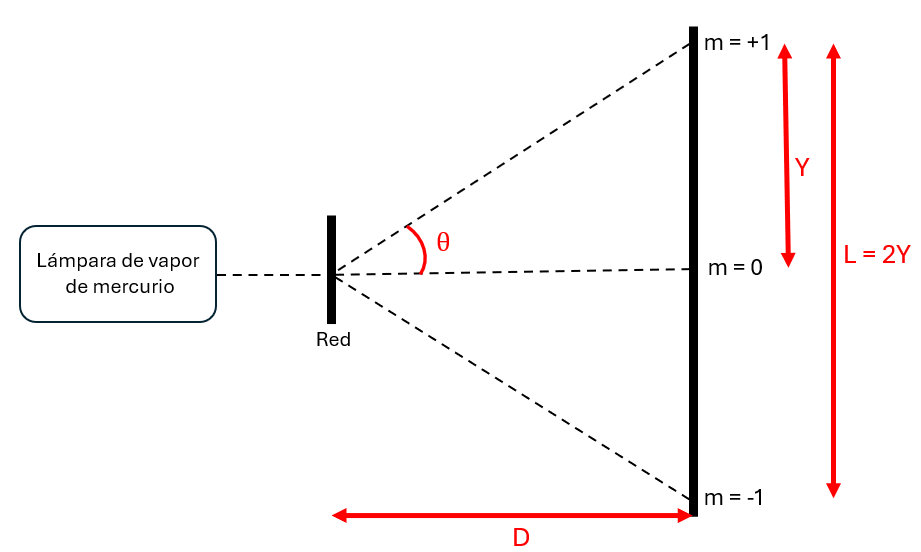
\includegraphics[width=0.5\columnwidth]{diagramaExperimental1.png}
        \caption{\label{fig1}Diagrama de la disposición experimental para calcular la constante de la red, junto con las variables intervinientes.
        }
\end{figure}

\subsection{Longitud de onda de las líneas azules, verdes y rojas}
Esta segunda parte del experimento tiene como objetivo determinar las longitudes de onda de los distintos componentes del haz emitido por la lámpara de mercurio. \par Se armó la disposición experimental igual que se hizo para la primera parte, con la adición de una pantalla blanca en el extremo opuesto a la lámpara de vapor, un diafragma contiguo a la lámpara y previo a la red, y una lente convergente contigua al diafragma y también previa a la red (ver figura 2).\par Se ajustó tanto la cantidad de luz que permitía pasar el diafragma, como su posición y la posición de la lente, de manera que las líneas de los máximos de interferencia de primer orden correspondientes a las distintas longitudes de onda se vieran con la mayor nitidez posible y sean a la vez lo más finitas posibles (para obtener mediciones más precisas). \par Finalmente, se midieron la distancia D entre la pantalla y la red, y las distancias $2Y_{azul}$, $2Y_{verde}$ y $2Y_{naranja}$ entre los máximos de primer orden de cada color (es decir, de cada longitud de onda).

\begin{figure}[!h] 
        \centering 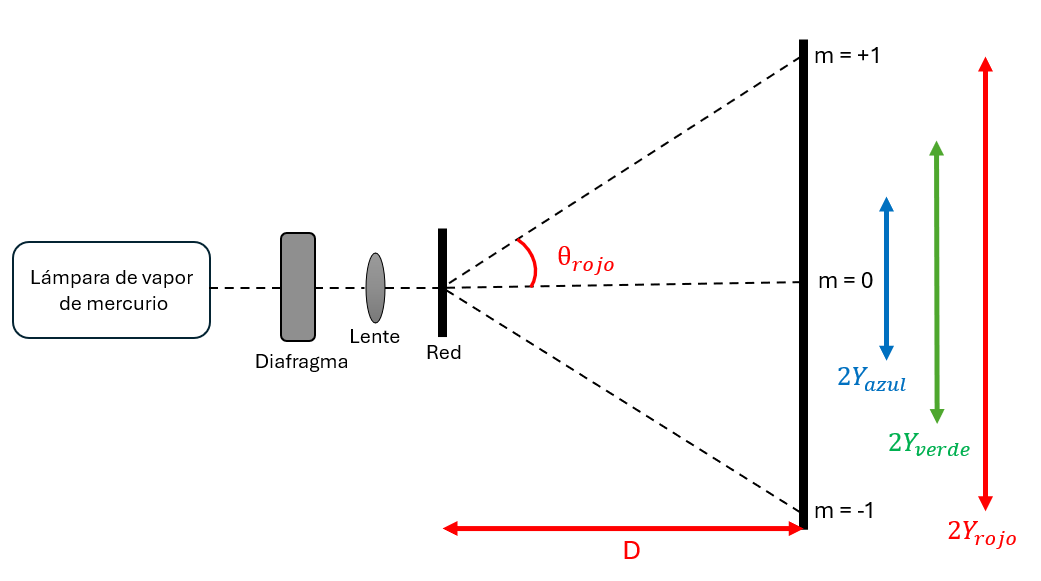
\includegraphics[width=0.5\columnwidth]{diagramaExperimental2.png}
        \caption{\label{fig2}Diagrama de la disposición experimental para calcular las longitudes de onda, junto con las variables intervinientes.
        }
\end{figure}

\begin{figure}[!h] 
        \centering 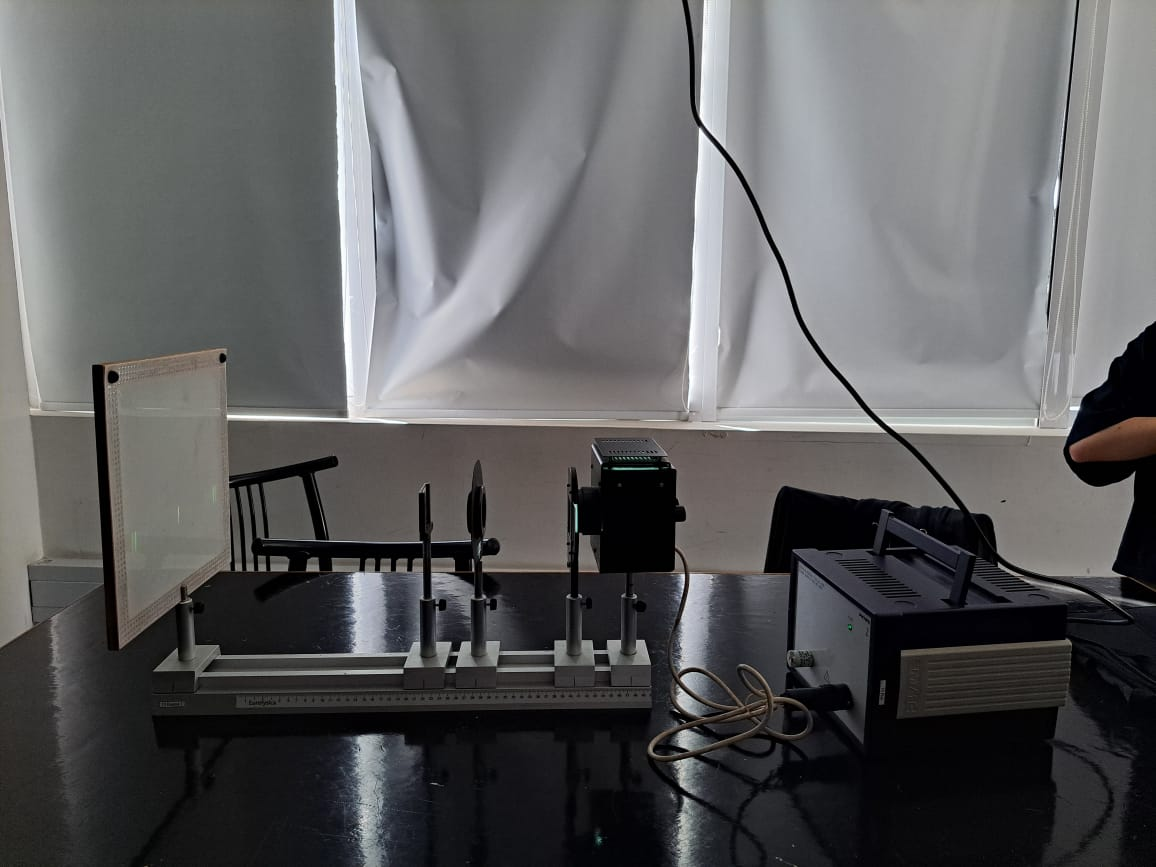
\includegraphics[width=0.5\columnwidth]{dispositivo3.jpg}
        \caption{\label{fig3}Foto de la disposición experimental en funcionamiento. De derecha a izquierda se pueden ver la fuente de alimentación, la lámpara de vapor de mercurio, el diafragma, la lente, la red de difracción y la pantalla.
        }
\end{figure}

\section{RESULTADOS (rita)}
Para más información sobre el desarrollo de las incertezas, ir al apéndice de incertezas, sección 6.

\subsection{Constante de la red}
Se midieron los valores 
\\ $D = (169 \pm 0,1)$ cm
\\ $2Y = (139,40 \pm 1)$ cm
\par Reemplazando en la ecuación (1) se obtiene que
\begin{center}
    $K = (6025 \pm 739) \frac{1}{cm}$
\end{center}

\subsection{Longitud de onda de las líneas azul, verde y roja}
Se midieron el valor $D = (29,60 \pm 0,1)$ cm y los presentados en la tabla 1:

\begin{table}[H]
  \centering
  \begin{tabular}{|c|c|}
  \hline
  Color & Y (cm) \\
  \hline
  $Azul$  & $7,9 \pm 0,1$  \\ \hline
  $Verde$  & $10,15 \pm 0,1$ \\ \hline
  $Amarillo$  & $10,75 \pm 0,1$ \\ \hline
  \end{tabular}
  \caption{\centering Valores de las distancias entre el máximo de primer orden y el de orden cero de cada longitud de onda (Y, no 2Y).}
  \label{tabla1}
\end{table}

Reemplazando en la ecuación (2) se obtienen las longitudes de onda presentadas en la tabla 2:

\begin{table}[H]
  \centering
  \begin{tabular}{|c|c|}
  \hline
  Onda por color & $\lambda $ (nm)  \\
  \hline
  ${\lambda_{azul}}$  & $ 428,3 \pm 52,7$  \\ \hline
  ${\lambda_{verde}}$  & $ 538,8 \pm 66,2 $ \\ \hline
  ${\lambda_{amarillo}}$  & $ 567,0 \pm 69,6 $\\ \hline
  \end{tabular}
  \caption{\centering Valores calculados de las longitudes de onda de tres colores. }
  \label{tabla2}
\end{table}

\section{CONCLUSIONES (ian)}

\section{APÉNDICE: Cálculo de Incertezas}
Entonces los valores buscados fueron los siguientes:

\subsection{Constante de la red}
Dado que en esta primera parte se considera el dato de la longitud de onda del haz emitido como un valor exacto, su incerteza es $\Delta \lambda$ nula y ${\Delta}K$ será:

\begin{equation}
  {\Delta}K = \sqrt{({\Delta}y)^2(\frac{D^{2}}{{\lambda} \left(Y^{2} + D^{2}\right)^{\frac{3}{2}}})^2+({\Delta}D)^2(-\frac{YD}{{\lambda} \left(D^{2} + Y^{2}\right)^{\frac{3}{2}}})^2}
\label{equation5}
\end{equation}

donde $\Delta y = \frac{\Delta L}{2}$. Como los máximos de interferencia "no son puntuales", la incerteza de esta medición no puede regirse acorde a la incerteza de la cinta métrica, por lo que se toma $\Delta L = $"diámetro del punto de luz"$\approx 2$ cm.

\subsection{ Longitud de onda de las líneas azul, verde y roja}
En esta segunda parte, sabemos que $\Delta D = 0,1$ cm.
Para calcular la incerteza de cada longitud de onda utilizamos la siguiente ecuación:
\begin{equation}
  {\Delta}{\lambda} = \sqrt{({\Delta}K)^2(-\frac{Y}{\sqrt{Y^{2} + 
  D^{2}} \, K^{2}})^2 + ({\Delta}D)^2(-\frac{YD}{K \left(D^{2} + Y^{2}\right)^{\frac{3}{2}}})^2+ ({\Delta}Y)^2(\frac{D^{2}}{K \left(Y^{2} + D^{2}\right)^{\frac{3}{2}}})^2}
\label{equation5}
\end{equation}
Se pueden ver los valores de cada incerteza junto a su respectiva longitud de onda en la tabla 2, en la sección de resultados.

\end{document}
